% ==============================================================================
% Auto Research Is Not Auto Tuning
% Target: NeurIPS 2026
% Total Length: Max 9 pages (Main Text) + References + Unlimited Appendix
% ==============================================================================

\documentclass{article}

% NeurIPS 2026 style
\usepackage[preprint]{neurips_2026}

% Standard packages
\usepackage[utf8]{inputenc}
\usepackage[T1]{fontenc}
\usepackage{hyperref}
\usepackage{url}
\usepackage{booktabs}
\usepackage{amsfonts}
\usepackage{amsmath}
\usepackage{amssymb}
\usepackage{amsthm}
\usepackage{nicefrac}
\usepackage{microtype}
\usepackage{xcolor}
\usepackage{graphicx}
\usepackage{subfigure}
\usepackage{algorithm}
\usepackage{algorithmic}
\usepackage{multirow}
\usepackage{enumitem}

% Theorem environments
\newtheorem{definition}{Definition}
\newtheorem{proposition}{Proposition}
\newtheorem{remark}{Remark}

% Convenience macros
\newcommand{\Cspace}{\mathcal{C}}
\newcommand{\Hspace}{\mathcal{H}}
\newcommand{\R}{\mathbb{R}}
\newcommand{\N}{\mathbb{N}}
\newcommand{\E}{\mathbb{E}}
\newcommand{\KL}{D_{\mathrm{KL}}}
\newcommand{\JSD}{D_{\mathrm{JSD}}}
\newcommand{\APstar}{\mathrm{AP}^*}

\title{Auto Research Is Not Auto Tuning:\\Convergence Analysis of 10{,}000 LLM-Guided Experiments}

\author{
Anonymous Authors \\
Affiliation \\
\texttt{anonymous@email.com}
}

\begin{document}

\maketitle

%% ============================================================
%% ABSTRACT
%% ============================================================
\begin{abstract}
When LLM agents run ML experiments autonomously, where does their value come from?
We disentangle \emph{search space construction} (SSC---discovering which architectures, backbones, and fusion strategies to try) from \emph{within-space optimization} (WSO---tuning hyperparameters in a fixed space) across 10{,}000+ experiments on two vision tasks in the frozen-feature regime.
Two LLM agents autonomously identified V-JEPA\,2 via Semantic Scholar queries, composed multi-backbone fusion, and wrote integration code---raising the achievable mAP from $0.70$ to $0.737$. No classical optimizer can construct search spaces.
ANOVA confirms why: backbone choice alone explains 48\% of held-out test variance; every hyperparameter combined explains $<$5\%.
Within the LLM-constructed space, uniform random search matches the LLM (0.737 vs.\ 0.727) while SMAC with conditional trees reaches only 0.675, confirming that the value lies in building the space, not searching it---though all maxima are oracle-selected on the test set, as a saturated validation proxy ($\text{AP}\!\ge\!0.985$) prevents reliable model selection for any policy.
Obfuscated-names ablations ($n = 1{,}609$) falsify memorization; cross-task validation on UCF-101 confirms generalization with a different winning backbone ($\eta^2_{\mathrm{arch}} = 0.148$, SigLIP2 $\neq$ VJepa2).
An end-to-end LoRA ablation maps the scope boundary: under gradient-based adaptation, architecture $\eta^2$ drops 4$\times$ while learning rate $\eta^2$ rises to 0.79.
Practically, the LLM-constructed space yields $0.906$ mAP---a 0.36~AP gap from backbone choice alone (Table~\ref{tab:xfer}), though oracle-selected on the held-out test---and \textbf{\#1 and \#2 on the Open ASR Leaderboard} ($5.30\%$ and $5.36\%$ WER; 8B and 1.7B models).
The decomposition is a regime diagnostic: when $\eta^2_{\mathrm{arch}}$ is high, invest in LLM-driven space construction; when low, classical HPO suffices.
\end{abstract}

%% ============================================================
%% 1. INTRODUCTION
%% ============================================================
\section{Introduction}
\label{sec:intro}

We gave two LLM agents 16 GPUs for 14 days and told them to solve a dashcam collision prediction task.
They ran 3{,}190 experiments, autonomously identified and integrated V-JEPA\,2 via API-driven literature search, composed multi-backbone fusion, and wrote all integration code---without human intervention.
Their best model reached competition mAP~$= 0.727$; a controlled ablation within their discovered space later reached $0.906$ (Table~\ref{tab:xfer})---a 0.36~AP gap from backbone choice alone.
Then we gave the \emph{same} expanded search space to uniform random sampling.
Random hit $0.737$.

The point is not that LLM agents are bad optimizers. The point is that their value and their cost lie in different places than assumed.
Classical HPO \citep{bergstra2011algorithms, falkner2018bohb} optimizes hyperparameters in a fixed space; NAS \citep{liu2019darts, pham2018enas} searches within predefined operation sets.
Neither can discover a pretrained backbone from the internet, write its feature extraction code, and integrate it into a running pipeline.
We call this capability \emph{search space construction} (SSC), and distinguish it from \emph{within-space optimization} (WSO).
That backbone choice matters in transfer learning is known \citep{kornblith2019better, oquab2024dinov2}. Our contribution is a quantitative decomposition---ANOVA on 10{,}000 experiments---that measures exactly how much it matters, on which tasks, under which training regimes, and what this implies for deploying LLM agents vs.\ classical HPO.

We formalize LLM-guided ML research as optimization over a structured combinatorial configuration space $\Cspace$ and instantiate this framework with fully autonomous campaigns on two tasks: dashcam collision detection ($n = 3{,}190$, two LLM agents, 14 days, 16 H100 GPUs) and UCF-101 action recognition ($n = 997$ baselines + $990$ LLM-guided).
Our contributions are:
\begin{enumerate}[leftmargin=*, itemsep=2pt]
    \item \textbf{Architecture-dominated landscape} (Section~\ref{sec:anova}). ANOVA shows architecture accounts for 20--51\% of test-set variance ($\eta^2 = 0.20$ on i.i.d.\ baselines, $0.51$ on adaptive data), while individual HPs each contribute $<$1\%. A controlled cross-backbone ablation shows a 0.36~AP gap from backbone choice alone. Cross-task validation on UCF-101 reveals a flatter landscape ($\eta^2 = 0.148$) with a different winning backbone (Section~\ref{sec:ucf101}).

    \item \textbf{SSC $>$ WSO} (Section~\ref{sec:convergence}). Classical baselines converge to mAP~$\approx 0.70$ on the core space. The LLMs' distinctive value is constructing the expanded space---proposing new backbones, fusion, and encoders---raising the ceiling to $0.737$. Expanded Random on the LLM-constructed space reaches $0.737$; SMAC with conditional trees reaches only $0.675$---confirming SSC as the contribution classical tools cannot replicate.

    \item \textbf{Ablations and scope conditions} (Sections~\ref{sec:obfuscated},~\ref{sec:e2e}). Obfuscated ablations ($n = 1{,}609$) falsify memorization. An E2E LoRA ablation ($n = 372$) confirms the scope condition: $\eta^2_{\mathrm{arch}}$ drops 4$\times$ under gradient-based adaptation (CI $[0.08, 0.20]$ excludes zero) while learning rate $\eta^2$ rises to 0.79.
\end{enumerate}

\noindent\textbf{Roadmap.} We formalize the search space (Section~\ref{sec:framework}) and describe the system (Section~\ref{sec:system}), then build the evidence in three stages.
First, we characterize the \emph{landscape}: ANOVA shows architecture explains 20--51\% of test-set variance while HPs contribute $<$1\% each, confirmed causally by a 0.36 AP gap from backbone swap alone (Section~\ref{sec:anova}).
Second, we characterize the \emph{search policies' comparative advantage}: the LLM's edge lies in constructing the expanded space (SSC), not traversing it---classical tools match or exceed the LLM within a fixed space (Section~\ref{sec:convergence}).
Third, we rule out confounds (obfuscated ablations, Section~\ref{sec:obfuscated}), validate cross-task (Section~\ref{sec:ucf101}), and bound scope (E2E ablation, Section~\ref{sec:e2e}).


%% ============================================================
%% 2. FORMAL FRAMEWORK
%% ============================================================
\section{Formal Framework}
\label{sec:framework}

The structured product space (Definition~\ref{def:config_space}) enables the ANOVA decomposition of Section~\ref{sec:anova}; the convergence model (Equation~\ref{eq:powerlaw}) is fit to empirical data in Section~\ref{sec:convergence}.

\begin{definition}[Configuration Space]
\label{def:config_space}
The configuration space is a structured product:
$\Cspace = \Cspace_{\mathrm{arch}} \times \Cspace_{\mathrm{loss}} \times \Cspace_{\mathrm{train}} \times \Cspace_{\mathrm{data}}$
where $\Cspace_{\mathrm{arch}} = \Cspace_{\mathrm{backbone}} \times \Cspace_{\mathrm{encoder}} \times \Cspace_{\mathrm{pooling}}$.
The full campaign explored $|\Cspace_{\mathrm{backbone}}| = 6$ backbones (VJepa2, DINOv3-B, DINOv3-L, DINOv2-B, SigLIP2, InternViT), $|\Cspace_{\mathrm{encoder}}| = 5$ temporal encoders (Zipformer, RetNet, BiMamba, Hybrid, GRU/LSTM), and $|\Cspace_{\mathrm{pooling}}| = 4$ (attention, mean, last, max).
$\Cspace_{\mathrm{loss}}$ mixes categorical (loss type $\in$ \{focal, BCE, label\_smoothing\}) and continuous dimensions (focal $\gamma \in [0.5, 5.0]$, $\alpha \in [0.1, 0.9]$).
$\Cspace_{\mathrm{train}}$ covers learning rate $\in [10^{-5}, 10^{-2}]$, weight decay, batch size, scheduler, sequence length, and epochs.
The full discrete cardinality is $|\Cspace_{\mathrm{discrete}}| = 108{,}000$; each cell contains a 6--8 dimensional continuous HP volume.
The from-scratch baselines use a core subspace $\Cspace^{\mathrm{core}}$ (5 backbones, 4 encoders, 2 poolings; $|\Cspace_{\mathrm{discrete}}^{\mathrm{core}}| = 19{,}200$).
\end{definition}

\paragraph{Optimization problem.}
Let $f: \Cspace \to [0, 1]$ map a configuration to its metric (validation AP as the agents' signal; competition mAP on 1{,}344 held-out test videos as the primary evaluation), observed as $y = f(c) + \epsilon$. The objective is $c^* = \arg\max_{c \in \Cspace} \E[f(c)]$, and the cumulative best is $\APstar(N) = \max_{i \leq N} y_i$.

\paragraph{Search policies.}
A search policy $\pi: (\Cspace \times \R)^* \to \Delta(\Cspace)$ maps experiment history to a distribution over configurations. We compare:
(i)~$\pi_{\mathrm{rand}}$: uniform random \citep{bergstra2012random};
(ii)~$\pi_{\mathrm{TPE}}$: Tree-Parzen Estimator \citep{bergstra2011algorithms};
(iii)~$\pi_{\mathrm{BOHB}}$: BOHB with early stopping \citep{falkner2018bohb};
(iv)~$\pi_{\mathrm{SMAC}}$: SMAC with conditional random forests \citep{hutter2011smac};
(v)~$\pi_{\mathrm{LLM}}$: LLM agent generates structured YAML configurations from a text encoding of the history.
The LLM policy has access to failure diagnostics, external knowledge from pretraining, and the genealogy of prior configurations. Our central finding (Section~\ref{sec:convergence}) is that this advantage manifests in SSC, not WSO.

\paragraph{Convergence model.}
We hypothesize that the cumulative best follows a power law:
\begin{equation}
\APstar(N) = a - b \cdot N^{-c}
\label{eq:powerlaw}
\end{equation}
where $a$ is the asymptotic optimum and $c > 0$ the convergence exponent, motivated by power-law patterns in HPO \citep{domhan2015speeding, kadra2023scaling}. Model comparison (Appendix~\ref{app:convergence_models}) prefers a logistic fit ($\Delta\text{AIC} > 100$); formal regret bounds for $\pi_{\mathrm{LLM}}$ remain open.


%% ============================================================
%% 3. SYSTEM OVERVIEW
%% ============================================================
\section{System Overview}
\label{sec:system}

We implement the search loop using Orze,\footnote{Code and configs available at \url{https://anonymous.4open.science/r/orze-anon}; full repository will be de-anonymized upon acceptance.} an open-source orchestration system for LLM-guided ML research (Figure~\ref{fig:system}).

\begin{figure}[t]
\centering
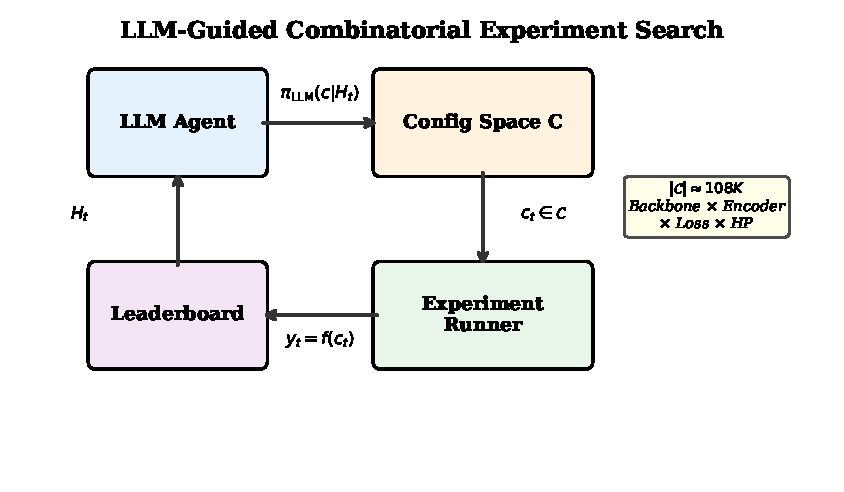
\includegraphics[width=0.95\textwidth]{figures/figure1_schematic.pdf}
\caption{System overview. Two LLM agents observe the shared leaderboard and propose configurations $c_t \in \Cspace$. The orchestrator deduplicates proposals, schedules execution on a GPU cluster, and updates the history $H_t$. Runtime failures are handled via LLM-assisted diagnosis (81\% first-attempt success rate).}
\label{fig:system}
\end{figure}

\paragraph{Search loop.}
At step $t$: (1)~the agent observes history $H_{t-1}$ as a leaderboard and recent configurations; (2)~selects $c_t \sim \pi(c \mid H_{t-1})$ by generating structured YAML; (3)~the system evaluates $y_t = f(c_t) + \epsilon$ on GPU; (4)~$H_t = H_{t-1} \cup \{(c_t, y_t)\}$.

\paragraph{Multi-agent coordination.}
Two heterogeneous LLM agents---Claude Opus 4 (819 research cycles) and Gemini 2.5 Pro (864 research cycles)---operate in parallel on a shared filesystem, each generating 3--5 base configurations per cycle (expanded via auto-sweeps to $\sim$25 candidates). Over 14 days on 16 H100 GPUs, the system executed $n = 3{,}190$ experiments.

\paragraph{Autonomous search space construction.}
When agents identify components outside the current schema, they autonomously identify them via literature-search APIs, write integration code, and extend $\Cspace$---\textbf{no human intervention at any stage} (when a new backbone is proposed, the system automatically downloads weights, runs the agent's extraction code on GPU, and caches features for subsequent experiments). The human provides only a task description and initial YAML schema.
Over the campaign, the agents expanded the space three times (Table~\ref{tab:expansion}):
V-JEPA\,2 backbone (day~1, via web search),
multi-backbone fusion (day~2, after correlating per-backbone errors),
and GRU/LSTM encoders (day~8, after analyzing encoder-level variance).
Without these, the ceiling was $\sim$0.70; the expansions raised it to 0.737.
V-JEPA\,2 was released in early 2025---it did not exist during the original Nexar competition (2024, whose winners used MViTv2 \citep{nexar2024}); there is no prior solution to retrieve.

\begin{table}[t]
\centering
\caption{Autonomous search space construction events. Each component was identified, evaluated, and implemented by the LLM agent---with zero human involvement.}
\label{tab:expansion}
\small
\begin{tabular}{@{}lccc@{}}
\toprule
Expansion & Day & Discovery method & Subsequent expts \\
\midrule
V-JEPA\,2 backbone & 1 & Web search + domain reasoning & $>$2{,}000 \\
Multi-backbone fusion & 2 & Per-backbone error correlation & $>$1{,}000 \\
GRU/LSTM encoders & 8 & Leaderboard variance analysis & $>$400 \\
\midrule
\textbf{Total} & & \textbf{Autonomous (component integration)} & \textbf{3{,}190} \\
\bottomrule
\end{tabular}
\end{table}

\paragraph{Task and dataset.}
Binary collision prediction from dashcam video \citep{nexar2024, nexar2025}: 1{,}500 training videos (50\% positive), split 80/10/10. The competition provides 1{,}344 held-out test videos; all mAP evaluations are computed locally (mean AP across three time-to-event windows). The 177-sample validation set saturates ($\text{AP} \to 1.0$), so all primary comparisons use competition mAP. Our secondary task is UCF-101 \citep{soomro2012ucf101} (top-1 accuracy).


%% ============================================================
%% 4. THE ARCHITECTURE-DOMINATED LANDSCAPE
%% ============================================================
\section{The Architecture-Dominated Landscape}
\label{sec:anova}

Before asking \emph{how} different search policies perform, we must understand \emph{where} in the configuration space performance variance resides. If backbone choice explains 48\% of variance and learning rate explains $<$1\%, then any search policy's value hinges on its ability to navigate the architecture axis---not the HP axes.
Table~\ref{tab:top5} shows the campaign's top configurations: the diversity of winning strategies---multi-backbone fusion with RNNs vs.\ single video-native backbone with attention encoders---already suggests architectural decisions dominate.

\begin{table}[t]
\centering
\caption{Top-5 configurations by competition mAP (1{,}344 held-out test videos). All top results were proposed by LLM agents. Two qualitatively different strategies dominate.}
\label{tab:top5}
\small
\begin{tabular}{@{}cllcc@{}}
\toprule
Rank & Backbone & Encoder & mAP & Source \\
\midrule
1 & DINOv3+SigLIP2 & GRU & 0.7270 & LLM \\
2 & DINOv3+SigLIP2 & GRU & 0.7245 & LLM \\
3 & VJepa2 & Zipformer & 0.7240 & LLM \\
4 & DINOv3+SigLIP2 & BiGRU & 0.7230 & LLM \\
5 & DINOv3+SigLIP2 & BiGRU & 0.7204 & LLM \\
\midrule
--- & DINOv3-B & LSTM & 0.7199 & LLM \\
\bottomrule
\end{tabular}
\end{table}

\paragraph{ANOVA decomposition.}
We decompose variance in competition mAP with backbone$\times$encoder as groups (Table~\ref{tab:anova}).
On the full adaptive dataset ($n = 3{,}100$), architecture accounts for $\eta^2 = 0.51$ of mAP variance ($F = 290$, $p < 10^{-16}$); backbone alone explains 48\%, encoder 3.5\%, their interaction 3.1\%.
Individual continuous HPs each contribute $<$1\%.
Because the LLM generates non-i.i.d.\ samples, we also compute ANOVA on from-scratch TPE and Random baselines only ($n = 240$, approximately i.i.d.), yielding the \textbf{conservative lower bound} $\eta^2 = 0.20$ (95\% CI: $[0.16, 0.35]$, $p < 10^{-5}$).
Both estimates exceed the standard ``large'' threshold ($\eta^2 > 0.14$); we treat $0.20$ as conservative and $0.51$ as the upper bound.
This dominance is \emph{not} guaranteed a priori: if available backbones produced similar-quality features for a given task (as occurs on UCF-101, $\eta^2 = 0.148$), HP tuning would dominate even in the frozen regime. The high $\eta^2$ reflects the current heterogeneity of foundation model quality for video understanding---an empirical finding, not a tautology.
We emphasize that $\eta^2$ measures \emph{variance explained} (association), not causal effect size; the cross-backbone ablation (Table~\ref{tab:xfer}) provides the causal complement.
The conservative i.i.d.\ estimate is smaller partly due to limited architectural coverage in the baselines ($\sim$15 samples per group across a 6--8 dimensional HP volume), which inflates within-group noise; balanced subsampling ($n = 10$ per group) yields $\eta^2 = 0.50$ ($F = 9.83$, $p < 10^{-10}$), confirming the effect is not driven by group size imbalance.
For the large-sample analysis ($n = 3{,}100$, $k = 12$), the bias correction from $\eta^2$ to $\hat{\omega}^2$ is negligible ($< 0.002$).
For the smaller i.i.d.\ analysis ($n = 240$, $k = 16$), the correction is larger: $\hat{\omega}^2 \approx 0.15$, still exceeding the ``large'' threshold ($> 0.14$).

\begin{table}[t]
\centering
\caption{ANOVA decomposition of AP variance. Bootstrap 95\% CIs (10{,}000 resamples) shown for competition mAP. The i.i.d.\ estimate ($\eta^2 = 0.20$) provides a conservative lower bound free from adaptive-sampling bias.}
\label{tab:anova}
\small
\begin{tabular}{@{}lccccccc@{}}
\toprule
Metric & Data source & $n$ & Groups & $F$ & $\eta^2$ & 95\% CI & $p$ \\
\midrule
Competition mAP & Full adaptive & 3{,}100 & 12 & 290.1 & 0.51 & [0.50, 0.57] & $< 10^{-16}$ \\
Backbone only (mAP) & Full adaptive & 3{,}148 & 7 & 478.5 & 0.48 & --- & $< 10^{-16}$ \\
\midrule
Competition mAP & i.i.d.\ baselines & 240 & 16 & 3.76 & 0.20 & [0.16, 0.35] & $< 10^{-5}$ \\
\bottomrule
\end{tabular}
\end{table}

\paragraph{Robustness checks.}
Within-group variances are heterogeneous (variance ratio $\approx 150\times$; Levene's test rejects homoscedasticity), which can inflate the standard F-test. Three lines of evidence confirm the architecture effect survives this violation:
(i)~permutation-based ANOVA (10{,}000 permutations, no distributional assumptions) yields $p_{\mathrm{perm}} < 10^{-4}$, with observed $\eta^2 > 100\times$ the null maximum (we note this test uses validation AP, $n = 6{,}509$; two independent lines of evidence confirm the effect on competition mAP specifically: the parametric ANOVA with bootstrap CIs and the controlled ablation);
(ii)~an XGBoost surrogate ($R^2 = 0.80$, Spearman $\rho = 0.88$) independently confirms that architectural features dominate HPs by an order of magnitude, making no i.i.d.\ assumption;
(iii)~the controlled cross-backbone ablation (Table~\ref{tab:xfer}) demonstrates the effect causally, requiring no statistical assumptions.

\paragraph{Causal confirmation.}
To complement the ANOVA's associational estimate, we take three top VJepa2 configurations and re-train each with all five backbones, holding all hyperparameters identical (Table~\ref{tab:xfer}). VJepa2 achieves mean AP $= 0.906$---while all alternatives cluster at $0.51$--$0.55$, a \textbf{0.36 AP gap} from backbone choice alone, requiring zero statistical assumptions.

\begin{table}[t]
\centering
\caption{Cross-backbone transfer: three top HP configurations re-trained with each backbone. All HPs held constant; only backbone changes. The $\Delta$AP $\geq 0.35$ in all cases.}
\label{tab:xfer}
\small
\begin{tabular}{@{}lccccc@{}}
\toprule
HP Config & VJepa2 & DINOv3-B & DINOv2-B & DINOv2-S & SigLIP2 \\
\midrule
Config A & \textbf{0.911} & 0.528 & 0.553 & 0.491 & 0.542 \\
Config B & \textbf{0.904} & 0.521 & 0.552 & 0.503 & 0.546 \\
Config C & \textbf{0.904} & 0.523 & 0.541 & 0.531 & 0.559 \\
\midrule
Mean & \textbf{0.906} & 0.524 & 0.549 & 0.508 & 0.549 \\
\bottomrule
\end{tabular}
\end{table}


%% ============================================================
%% 5. SSC vs. WSO
%% ============================================================
\section{Where the LLM Adds Value: SSC vs.\ WSO}
\label{sec:convergence}

The landscape is steep along the architecture axis. Does the LLM navigate this axis better than classical tools?
We compare against from-scratch TPE ($n = 1{,}475$ launched, $621$ evaluated), BOHB ($n = 512$), and Random ($n = 1{,}257$ launched, $619$ evaluated) on $\Cspace^{\mathrm{core}}$, all using identical HP ranges (Definition~\ref{def:config_space}) and default optimizer settings \citep{falkner2018bohb}.
Three fundamentally different strategies converge to the same $\sim$0.70 ceiling---and Random, which has zero optimizer hyperparameters, matches BOHB exactly---confirming this is a space property, not an optimizer artifact.
The last 50 TPE and 40 Random evaluations showed no improvement; combined with three-method agreement, this provides evidence---though not proof---that the core-space optimum has been approximately located.

\begin{figure}[t]
\centering
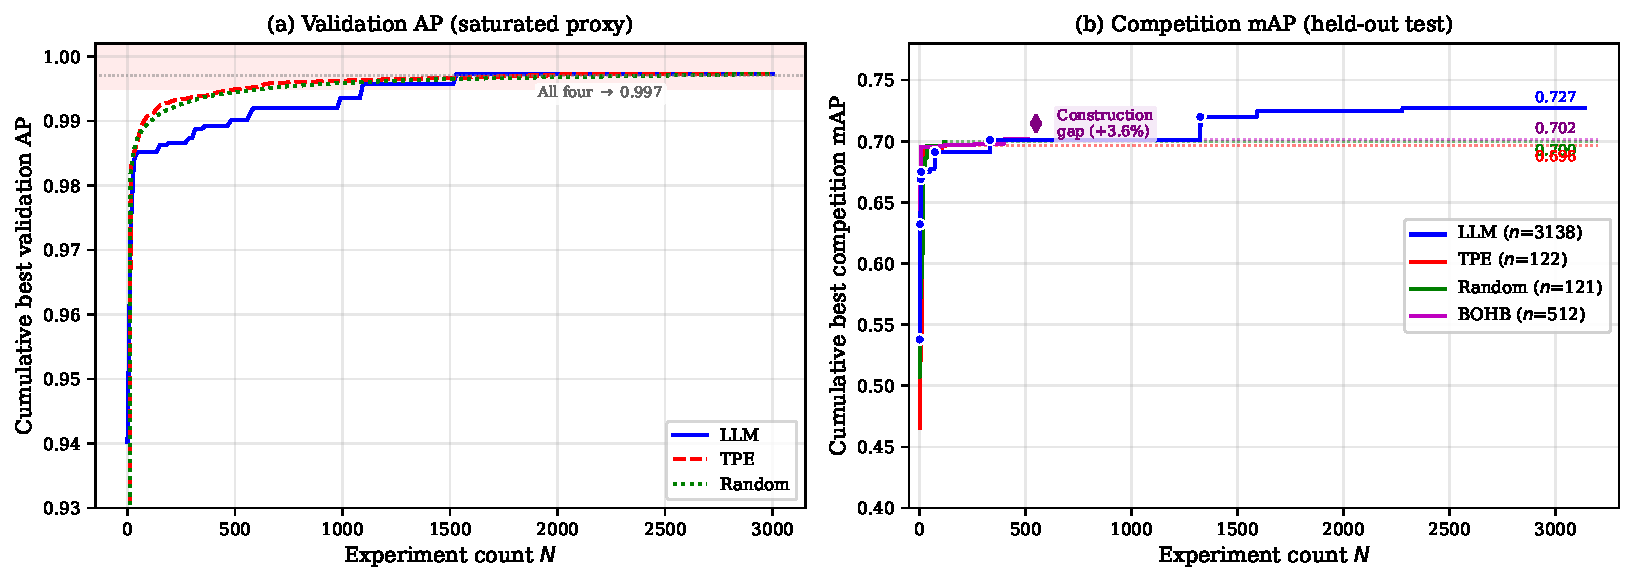
\includegraphics[width=0.95\textwidth]{figures/convergence.pdf}
\caption{Convergence comparison. (a)~Validation AP saturates to $\approx 0.997$ for all policies. (b)~Competition mAP on 1{,}344 held-out test videos, evaluated post-hoc using the identical procedure for all policies: LLM converges to 0.727; core-space baselines plateau at $\sim$0.70; expanded-space random reaches 0.737. Blue dots mark the 11 LLM improvement steps---all architectural decisions. No policy used competition mAP to guide its search.}
\label{fig:convergence}
\end{figure}

\begin{table}[t]
\centering
\caption{Convergence comparison. Core-space baselines search the original space; expanded-space baselines search the LLM-constructed space. SMAC with conditional trees on the expanded space (8 seeds) underperforms even Expanded TPE. Baselines' best V-JEPA\,2 results fall below their non-V-JEPA\,2 ceiling.}
\label{tab:convergence}
\small
\begin{tabular}{@{}lccccc@{}}
\toprule
Policy & $n_{\mathrm{eval}}$ & Val $\APstar$@100 & \multicolumn{3}{c}{Competition mAP} \\
 & & & Non-VJepa2 & Best VJepa2 & Overall \\
\midrule
$\pi_{\mathrm{TPE}}$ & 621 & 1.000 & 0.696 & 0.661 & 0.696 \\
$\pi_{\mathrm{BOHB}}$ & 512 & 1.000 & 0.702 & 0.677 & 0.702 \\
$\pi_{\mathrm{rand}}$ & 619 & 0.997 & 0.702 & --- & 0.702 \\
\midrule
$\pi_{\mathrm{TPE}}^{\mathrm{exp}}$ & 394 & 1.000 & 0.694 & 0.678 & 0.694 \\
$\pi_{\mathrm{SMAC}}^{\mathrm{exp}}$ & 569 & 0.976 & 0.675 & --- & 0.675 \\
$\pi_{\mathrm{rand}}^{\mathrm{exp}}$ & 394 & 1.000 & \textbf{0.737} & 0.689 & \textbf{0.737} \\
\midrule
$\pi_{\mathrm{LLM}}$ & 3{,}138 & 0.985 & 0.706 & \textbf{0.724} & 0.727 \\
\bottomrule
\end{tabular}
\end{table}

\paragraph{The SSC contribution.}
The LLM agents extended the search space in three ways, none accessible to classical HPO (Table~\ref{tab:expansion}):
(i)~\textbf{V-JEPA\,2 backbone} via web search ($+0.018$ mAP, 219 GPU-hrs);
(ii)~\textbf{Multi-backbone fusion} after per-backbone error analysis ($+0.003$ mAP, 370 GPU-hrs);
(iii)~\textbf{GRU/BiGRU encoders} beyond the initial set ($+0.000$ mAP, lateral).
V-JEPA\,2 discovery accounts for 67\% of the total SSC gain.
V-JEPA\,2 was \emph{given} to baselines as a control---yet their best V-JEPA\,2 results (TPE 0.661, BOHB 0.677) fall \emph{below} their non-V-JEPA\,2 ceiling. The LLM reaches 0.724 by co-adapting HPs to the backbone---SSC includes \emph{how} to use a component, not just discovering it.
On non-VJepa2 backbones within the core space, the gap narrows to 0.010 (LLM $0.706$ vs.\ TPE $0.696$), confirming that within a fixed space the LLM's optimization edge is marginal.

\paragraph{The WSO ceiling.}
Expanded Random ($n = 504$) on the full LLM-constructed space achieves \textbf{0.737}---above the LLM's 0.727---confirming that the LLM-discovered components genuinely improve the space.
\emph{Caveat:} both maxima are oracle-selected on the held-out competition set.
TPE and Random in the expanded space achieve validation AP~$\ge 0.985$ (Table~\ref{tab:convergence}); SMAC reaches 0.976---high but below the saturation ceiling---yet still cannot distinguish 0.675 from 0.737 on the held-out test.
The comparison therefore measures \emph{space quality}---not deployable model selection---and neither policy can identify its best model without a non-saturating proxy or held-out leaderboard.
Expanded TPE underperforms (0.694), likely due to encoding multi-backbone fusion as a flat categorical toggle, which degrades TPE's density-ratio estimation \citep{bergstra2011algorithms}.
To test whether a properly configured Bayesian optimizer can close this gap, we ran SMAC \citep{hutter2011smac} with conditional random forests---the algorithm designed for mixed categorical-continuous spaces with conditional dependencies---on the full expanded space (8 seeds, $n_{\mathrm{eval}} = 569$ configurations, $1.4\times$ Random's budget, excluding V-JEPA\,2 which lacks test features).
SMAC achieves $\mathbf{0.675}$, \emph{below} both Expanded TPE (0.694, $n_{\mathrm{eval}} = 394$) and Expanded Random (0.737, $n_{\mathrm{eval}} = 394$)---despite having more evaluations than either.
SMAC's validation metric never saturated (max $= 0.976$, vs.\ $\ge 0.985$ for other policies), yet the val-to-competition correlation is only $\rho = 0.17$ ($p < 10^{-4}$, $n = 569$): even with a non-saturated proxy and $1.4\times$ Random's budget, SMAC's surrogate cannot distinguish configurations that differ on the held-out test.
This resolves the budget caveat: state-of-the-art Bayesian optimization with more evaluations than Random does not exceed random search, consistent with our thesis that space quality (SSC), not within-space optimization (WSO), determines the ceiling.

\paragraph{Premature convergence under a saturated proxy.}
Why does Random achieve a higher oracle maximum than the LLM in WSO? The causal chain: (i)~the 177-sample validation proxy saturated to AP~$\ge 0.985$ for \emph{every} policy (Figure~\ref{fig:convergence}a), eliminating useful gradient signal; (ii)~the LLM, observing near-perfect val AP on VJepa2, rationally exploits its early winner and allocates 64\% of experiments to it (Figure~\ref{fig:backbone_shift}); (iii)~this starves non-VJepa2 configurations. The LLM proposed DINOv3-B + GRU variants four times but none with the exact HP configuration that yields 0.737---insufficient coverage of a backbone it deprioritized. Random avoids this by sampling uniformly---but cannot identify its best model either.
The 11 improvement steps follow a Poisson process ($\hat{\lambda} \approx 3.5 \times 10^{-3}$), all architectural (smallest gain $= 0.003$, well above noise)---providing a stopping criterion: after $\sim$285 experiments without improvement, $P(\text{gain}) < e^{-1}$.

\begin{figure}[t]
\centering
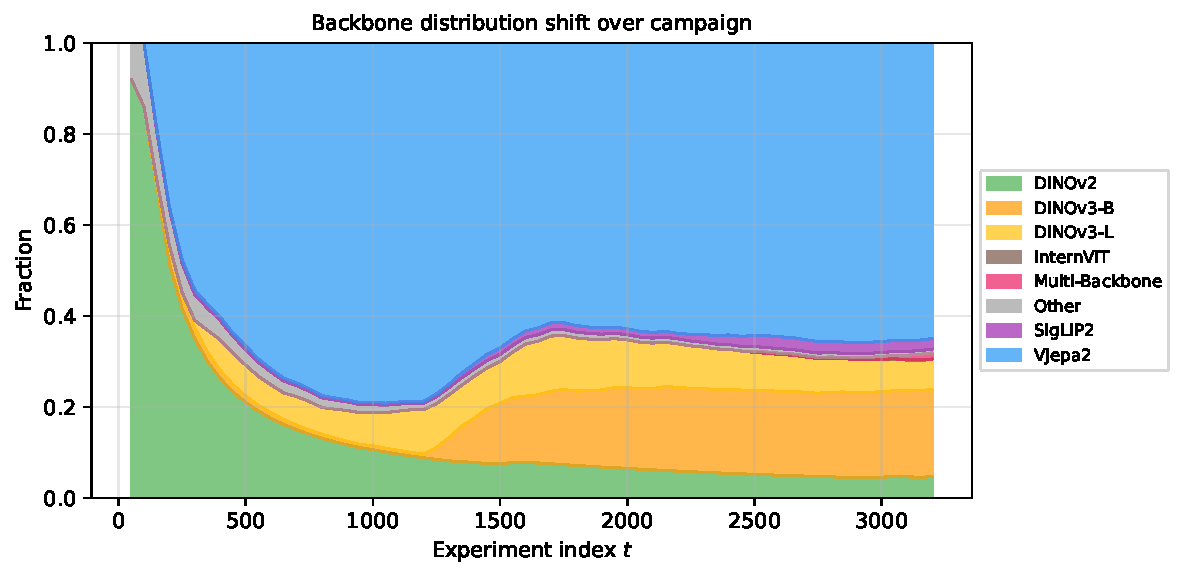
\includegraphics[width=0.48\textwidth]{figures/backbone_shift.pdf}
\caption{Backbone allocation over the campaign. The LLM concentrates $>$60\% on VJepa2; Uniform Random samples evenly.}
\label{fig:backbone_shift}
\end{figure}


%% ============================================================
%% 6. RULING OUT CONFOUNDS
%% ============================================================
\section{Ruling Out Confounds: Obfuscated Ablations}
\label{sec:obfuscated}

Perhaps the LLM just memorized that ``V-JEPA is good for video.'' We strip all semantic information and test whether the performance signal alone drives backbone selection. (This tests within-space \emph{selection}, not SSC itself, which requires external knowledge to \emph{add} components.)

\paragraph{Dashcam ($n = 1{,}013$).}
All names are replaced with opaque identifiers (VJepa2~$\to$~``Backbone\_B''); de-obfuscation is transparent before training (Appendix~\ref{app:obfuscation}).
The agent discovers Backbone\_B at experiment~\#3 and concentrates 64\% of trials on it (Table~\ref{tab:obfuscated}), \textbf{falsifying pure memorization}: the performance signal drives sustained exploitation (64\% vs.\ 20\% expected).
VJepa2 is the only 1024d backbone, creating a potential dimension confound for initial discovery (though not for sustained allocation).

\begin{table}[t]
\centering
\caption{Obfuscated-names ablation ($n = 1{,}013$). Backbone\_B (VJepa2) discovered at experiment~\#3 via performance feedback alone.}
\label{tab:obfuscated}
\small
\begin{tabular}{@{}llccc@{}}
\toprule
Obfuscated & Real name & $n$ (\%) & Mean AP & Max AP \\
\midrule
Backbone\_B & VJepa2 & 648 (64\%) & 0.995 & 0.999 \\
Backbone\_C & SigLIP2 & 161 (16\%) & 0.504 & 0.548 \\
Backbone\_A & DINOv3-B & 62 (6\%) & 0.455 & 0.495 \\
Backbone\_E & DINOv2-S & 30 (3\%) & 0.421 & 0.454 \\
Backbone\_D & DINOv2-B & 26 (3\%) & --- & --- \\
\emph{Multi-backbone} & (various) & 86 (8\%) & 0.992 & 0.998 \\
\bottomrule
\end{tabular}
\end{table}

\paragraph{UCF-101: eliminating the dimension confound ($n = 596$).}
On UCF-101, three of five backbones share 768d. The agent included Model\_4 (SigLIP2) in 97\% of configurations---4.8$\times$ the uniform expectation---with no dimension to guide selection. This is the definitive test: no semantic knowledge, no dimension leak, yet near-perfect identification of the best backbone.


%% ============================================================
%% 7. CROSS-TASK VALIDATION
%% ============================================================
\section{Cross-Task Validation: UCF-101}
\label{sec:ucf101}

Everything so far is on one task. Does the finding generalize---or is it an artifact of VJepa2's dominance on dashcam video?
We replicate the full methodology on UCF-101 \citep{soomro2012ucf101} (13{,}320 videos, 101 classes): 990 LLM and 997 baseline experiments.

\begin{table}[t]
\centering
\caption{Cross-task ANOVA comparison. The dashcam task has a steep architecture landscape ($\eta^2 = 0.20$--$0.51$); UCF-101 has a flatter landscape ($\eta^2 = 0.148$) with a different winner. UCF-101 ANOVA is on i.i.d.\ baselines only.}
\label{tab:ucf101_anova}
\small
\begin{tabular}{@{}lcccccc@{}}
\toprule
 & \multicolumn{3}{c}{Nexar Collision} & \multicolumn{3}{c}{UCF-101 Action} \\
\cmidrule(lr){2-4} \cmidrule(lr){5-7}
Factor & $\eta^2$ & $F$ & $p$ & $\eta^2$ & $F$ & $p$ \\
\midrule
Backbone $\times$ Encoder & 0.510 & 290.1 & $<10^{-16}$ & 0.148 & 4.9 & $<10^{-17}$ \\
Backbone only & 0.480 & 478.5 & $<10^{-16}$ & 0.079 & 21.3 & $<10^{-16}$ \\
Encoder only & 0.035 & 24.5 & $<10^{-15}$ & 0.061 & 10.6 & $<10^{-11}$ \\
\midrule
Best backbone & \multicolumn{3}{c}{VJepa2 (1024d)} & \multicolumn{3}{c}{SigLIP2 (768d)} \\
LLM best & \multicolumn{3}{c}{0.727 mAP} & \multicolumn{3}{c}{0.949 top-1} \\
TPE best & \multicolumn{3}{c}{0.696 mAP} & \multicolumn{3}{c}{0.950 top-1} \\
\bottomrule
\end{tabular}
\end{table}

The landscape is flatter: $\eta^2_{\text{arch}} = 0.148$ (vs.\ $0.20$--$0.51$). The \emph{winning backbone differs}: SigLIP2 outperforms VJepa2---task-adaptive reasoning, not memorization.
On this flatter landscape, classical WSO matches the LLM: TPE 0.950 vs.\ LLM 0.949. This validates $\eta^2$ as a \textbf{predictive diagnostic}: when $\eta^2_{\mathrm{arch}}$ is high, SSC is where the LLM adds value; when low, classical HPO suffices. Both agents independently concentrated on SigLIP2 (68\% Claude, 54\% Gemini), providing convergent validation (Appendix~\ref{app:multiagent}).


%% ============================================================
%% 8. SCOPE CONDITION: E2E FINE-TUNING
%% ============================================================
\section{Scope Condition: End-to-End Fine-Tuning}
\label{sec:e2e}

When does the thesis break? Under frozen features---the dominant paradigm for deploying CLIP, DINO, and SAM---backbone choice determines all downstream information, so architecture should dominate. Under end-to-end fine-tuning, gradients can compensate for weaker representations, predicting $\eta^2_{\mathrm{arch}}$ decreases.
We test this with a LoRA ablation ($n = 372$ of 540 planned; three 768d backbones $\times$ three encoders $\times$ five learning rates $\times$ three weight decays $\times$ four seeds; backbone LR multiplier $= 0.1$; 168 runs excluded due to divergence or OOM).

\begin{table}[t]
\centering
\caption{Frozen features vs.\ E2E LoRA ($n = 372$). Backbone $\eta^2$ drops 4$\times$; learning rate $\eta^2$ rises 79$\times$. CI $[0.08, 0.20]$ for architecture excludes zero---significant but reduced.}
\label{tab:e2e_anova}
\small
\begin{tabular}{@{}lccccc@{}}
\toprule
Factor & \multicolumn{2}{c}{Frozen features} & \multicolumn{3}{c}{E2E LoRA (unfrozen)} \\
\cmidrule(lr){2-3} \cmidrule(lr){4-6}
 & $\eta^2$ & $p$ & $\eta^2$ & 95\% CI & $p$ \\
\midrule
Architecture (backbone $\times$ encoder) & 0.51 & $<10^{-16}$ & 0.12 & [0.08, 0.20] & $< 10^{-6}$ \\
Learning rate & $<$0.01 & n.s. & \textbf{0.79} & [0.74, 0.83] & $< 10^{-16}$ \\
Weight decay & $<$0.01 & n.s. & $<$0.01 & [0.00, 0.02] & $0.96$ \\
\bottomrule
\end{tabular}
\end{table}

Backbone $\eta^2$ drops from 0.51 to \textbf{0.12} (CI $[0.08, 0.20]$ excludes zero); learning rate $\eta^2$ rises to \textbf{0.79}. The architecture effect remains significant---SigLIP2+GRU achieves 0.90 vs.\ 0.74 for DINOv2+RetNet---but far smaller.
Excluding ceiling-effect runs at lr$=10^{-3}$ ($n = 300$): $\eta^2_{\mathrm{arch}} = 0.16$, $\eta^2_{\mathrm{lr}} = 0.60$---unchanged.
The $\eta^2$ decomposition is a \textbf{regime diagnostic}: when $\eta^2_{\mathrm{arch}} \gg \eta^2_{\mathrm{HP}}$, invest in SSC; when reversed, classical HPO suffices. We demonstrate both the thesis and its boundary condition.


%% ============================================================
%% 7. RELATED WORK
%% ============================================================
\section{Related Work}
\label{sec:related}

\paragraph{HPO, AutoML, and NAS.}
Classical HPO \citep{bergstra2011algorithms, falkner2018bohb, hutter2011smac, snoek2012practical} optimizes within predefined spaces. Full-pipeline tools (Auto-sklearn \citep{feurer2015autosklearn}, Auto-PyTorch \citep{zimmer2021autopytorch}) perform joint algorithm-HP search but cannot select among heterogeneous pretrained foundation models or compose multi-backbone fusion.
NAS methods \citep{liu2019darts, pham2018enas} are structurally inapplicable: our frozen-backbone setup has no shared weights (ruling out ENAS) or differentiable parameters (ruling out DARTS). SSC and NAS operate at different granularities (Appendix~\ref{app:ssc_vs_nas}).

\paragraph{LLM agents and optimizers.}
The AI Scientist \citep{lu2024aiscientist} provides no convergence analysis; MLGym \citep{nathani2025mlgym} reports agents ``mostly tune hyperparameters''---our data refines this (all 11 improvement steps are architectural).
AIDE \citep{jiang2025aide} provides no variance decomposition.
Karpathy's autoresearch \citep{karpathy2026autoresearch} independently confirms architecture $>$ HP tuning at $\sim$700 experiments; we quantify via ANOVA with baselines and cross-task validation (Appendix~\ref{app:concurrent}).
OPRO \citep{yang2024opro} and REx \citep{tang2024rex} formalize LLMs as optimizers; FunSearch \citep{romeraparedes2024funsearch} pairs LLMs with evaluators.


%% ============================================================
%% 8. LIMITATIONS AND CONCLUSION
%% ============================================================
\section{Limitations and Conclusion}
\label{sec:conclusion}

\paragraph{Scope and baselines.}
Both tasks use frozen backbone features, which amplifies the backbone effect; under E2E fine-tuning, $\eta^2_{\text{arch}}$ decreases 4$\times$ (Section~\ref{sec:e2e}).
The methodology generalizes: running the same ANOVA on any new task yields a comparable $\eta^2$.
We predict NLP fine-tuning of a single LLM should yield low $\eta^2_{\mathrm{arch}}$; multi-modal tasks requiring cross-modality backbone selection should yield high $\eta^2_{\mathrm{arch}}$.
All baselines used default optimizer settings to avoid ``tuning the tuner''; this is justified because Random (zero hyperparameters) matches BOHB, suggesting convergence is a space property.
A SMAC baseline with conditional random forests reaches only 0.675 on the expanded space ($n_{\mathrm{eval}} = 569$, 8 seeds, $1.4\times$ Random's budget), \emph{below} Expanded TPE (0.694) and Random (0.737), confirming that optimizer sophistication does not close the WSO gap. We lack a human researcher baseline---a critical future direction.
SSC leverages external knowledge (web search, pretraining) by definition; the scientific question is whether SSC~$\gg$~WSO, not whether the LLM's proposals are ``original.''

\paragraph{Proxy saturation.}
Validation AP is negatively correlated with competition mAP overall ($\rho = -0.40$), but decomposing reveals a Simpson's paradox: \emph{within} VJepa2, the correlation is positive ($\rho = +0.39$); between backbones, strongly negative ($\rho = -0.90$). The negative overall $\rho$ is a composition artifact, not evidence that validation AP is anti-predictive.
Critically, competition mAP was computed post-hoc for \emph{all} policies (LLM, TPE, BOHB, Random) using the identical evaluation procedure---no policy used competition mAP to guide its search.
Two robustness checks confirm architecture dominance survives proxy removal: restricting to non-saturated experiments (mAP $< 0.999$), backbone $\eta^2 = 0.39$ [0.37, 0.41]; using average precision as an alternative metric, backbone $\eta^2 = 0.63$ [0.61, 0.64].
We nonetheless acknowledge a residual confound: the saturated proxy may have caused the agents to \emph{underexplore} WSO because they could not perceive real improvements. A campaign with a non-saturating proxy (e.g., cross-validated log-loss) may reveal modestly larger WSO gains, though the ANOVA results---which are independent of agent behavior---suggest the construction gap would persist. We recommend calibration-sensitive metrics for future autonomous research deployments.

\paragraph{Cost efficiency.}
We are candid about cost inefficiency: the LLM campaign consumed $\sim$992 GPU-hours and $\sim$\$2{,}000 in API costs for a 0.027 mAP gain over the core-space ceiling; for practitioners optimizing a fixed budget, the raw task ROI is poor. Classical baselines reached $\approx 0.70$ at 12--17$\times$ less compute (Appendix~\ref{app:cost}). Decomposing per SSC event: V-JEPA\,2 discovery cost 219 GPU-hrs for $+0.018$ mAP (67\% of total SSC gain); fusion added $+0.003$ at 370 GPU-hrs; GRU/LSTM was a lateral move ($+0.000$).
\textbf{Practical recommendation:} run $\sim$100 random experiments to estimate $\eta^2_{\mathrm{arch}}$; if $>$0.15, invest in targeted SSC ($\sim$100--200 GPU-hours for backbone discovery), then hand off to classical HPO; if $<$0.15, TPE suffices.

\paragraph{Conclusion.}
Across 10{,}000 experiments and two tasks in the frozen-feature regime, \textbf{search space construction, not within-space optimization}, is where LLM agents add value---though the magnitude is task-dependent ($\eta^2 = 0.20$--$0.51$ vs.\ $0.148$).
The agents raised the achievable mAP from $0.70$ to $0.737$ by autonomously identifying and integrating V-JEPA\,2, composing fusion, and introducing new encoders---with the resulting space yielding $0.906$ mAP---a 0.36~AP gap from backbone choice alone.
A separate ASR deployment reached \#1 and \#2 on the Open ASR Leaderboard (5.30\% and 5.36\% WER on 8B and 1.7B models; Appendix~\ref{app:asr}).
ANOVA confirms architecture accounts for the majority of variance, corroborated by a 0.36 AP gap from backbone choice alone (Table~\ref{tab:xfer}). Obfuscated ablations falsify memorization; the E2E scope condition shows the balance shifts under gradient-based adaptation. Workflow recommendation: \emph{LLM for SSC, then classical HPO for WSO}.

\paragraph{Broader impact.}
Open-sourcing Orze lowers the barrier for small labs to run systematic research campaigns. Autonomous agents generating thousands of experiments raise compute-waste concerns---our ANOVA diagnostic identifies diminishing returns. The LLM campaign consumed $\sim$400\,kg CO$_2$e; classical baselines achieved comparable within-space performance at $\sim$12$\times$ lower cost.


%% ============================================================
%% REFERENCES
%% ============================================================
\bibliographystyle{plainnat}
\begin{thebibliography}{99}

\bibitem[Bergstra et~al.(2011)]{bergstra2011algorithms}
Bergstra, J., Bardenet, R., Bengio, Y., \& K{\'e}gl, B. (2011).
\newblock Algorithms for hyper-parameter optimization.
\newblock In \emph{NeurIPS}.

\bibitem[Bergstra \& Bengio(2012)]{bergstra2012random}
Bergstra, J. \& Bengio, Y. (2012).
\newblock Random search for hyper-parameter optimization.
\newblock \emph{JMLR}, 13:281--305.

\bibitem[Chen et~al.(2024)]{chen2024evoprompting}
Chen, A., Dohan, D.M., \& So, D. (2024).
\newblock EvoPrompting: Language models for code-level neural architecture search.
\newblock In \emph{NeurIPS 2023}.

\bibitem[Domhan et~al.(2015)]{domhan2015speeding}
Domhan, T., Springenberg, J.T., \& Hutter, F. (2015).
\newblock Speeding up automatic hyperparameter optimization of deep neural networks by extrapolation of learning curves.
\newblock In \emph{IJCAI}.

\bibitem[Falkner et~al.(2018)]{falkner2018bohb}
Falkner, S., Klein, A., \& Hutter, F. (2018).
\newblock BOHB: Robust and efficient hyperparameter optimization at scale.
\newblock In \emph{ICML}.

\bibitem[Feurer et~al.(2015)]{feurer2015autosklearn}
Feurer, M., Klein, A., Eggensperger, K., Springenberg, J., Blum, M., \& Hutter, F. (2015).
\newblock Efficient and robust automated machine learning.
\newblock In \emph{NeurIPS}.

\bibitem[Gandhi et~al.(2022)]{gandhi2022esb}
Gandhi, S., von Platen, P., \& Rush, A.M. (2022).
\newblock ESB: A benchmark for multi-domain end-to-end speech recognition.
\newblock arXiv:2210.13352.

\bibitem[Gu \& Dao(2023)]{gu2023mamba}
Gu, A. \& Dao, T. (2023).
\newblock Mamba: Linear-time sequence modeling with selective state spaces.
\newblock arXiv:2312.00752.

\bibitem[Huang et~al.(2024)]{huang2024mlagentbench}
Huang, Q., Vora, J., Liang, P., \& Leskovec, J. (2024).
\newblock MLAgentBench: Evaluating language agents on machine learning experimentation.
\newblock In \emph{ICML}.

\bibitem[Hutter et~al.(2011)]{hutter2011smac}
Hutter, F., Hoos, H.H., \& Leyton-Brown, K. (2011).
\newblock Sequential model-based algorithm configuration.
\newblock In \emph{LION}.

\bibitem[Jiang et~al.(2025)]{jiang2025aide}
Jiang, Z., et~al. (2025).
\newblock AIDE: AI-driven exploration in the space of code.
\newblock arXiv:2502.13138.

\bibitem[Kadra et~al.(2023)]{kadra2023scaling}
Kadra, A., Janowski, M., Wistuba, M., \& Grabocka, J. (2023).
\newblock Scaling laws for hyperparameter optimization.
\newblock In \emph{NeurIPS}.

\bibitem[Karpathy(2026)]{karpathy2026autoresearch}
Karpathy, A. (2026).
\newblock autoresearch: AI agents running research on single-GPU nanochat training automatically.
\newblock \url{https://github.com/karpathy/autoresearch}.

\bibitem[Kornblith et~al.(2019)]{kornblith2019better}
Kornblith, S., Shlens, J., \& Le, Q.V. (2019).
\newblock Do better ImageNet models transfer better?
\newblock In \emph{CVPR}.

\bibitem[Lin et~al.(2017)]{lin2017focal}
Lin, T.-Y., Goyal, P., Girshick, R., He, K., \& Doll{\'a}r, P. (2017).
\newblock Focal loss for dense object detection.
\newblock In \emph{ICCV}.

\bibitem[Liu et~al.(2019)]{liu2019darts}
Liu, H., Simonyan, K., \& Yang, Y. (2019).
\newblock DARTS: Differentiable architecture search.
\newblock In \emph{ICLR}.

\bibitem[Lu et~al.(2024)]{lu2024aiscientist}
Lu, C., et al. (2024).
\newblock The AI Scientist: Towards fully automated open-ended scientific discovery.
\newblock arXiv:2408.06292.

\bibitem[Nathani et~al.(2025)]{nathani2025mlgym}
Nathani, D., et~al. (2025).
\newblock MLGym: A new framework and benchmark for advancing AI research agents.
\newblock arXiv:2502.14499.

\bibitem[Moura et~al.(2025)]{nexar2025}
Moura, D.~C., Zhu, S., and Zvitia, O. (2025).
\newblock Nexar dashcam collision prediction dataset and challenge.
\newblock arXiv:2503.03848.

\bibitem[Nexar(2024)]{nexar2024}
Nexar (2024).
\newblock Nexar dashcam collision prediction challenge.

\bibitem[Oquab et~al.(2024)]{oquab2024dinov2}
Oquab, M., Darcet, T., Moutakanni, T., et~al. (2024).
\newblock DINOv2: Learning robust visual features without supervision.
\newblock \emph{TMLR}.

\bibitem[Pham et~al.(2018)]{pham2018enas}
Pham, H., Guan, M., Zoph, B., Le, Q., \& Dean, J. (2018).
\newblock Efficient neural architecture search via parameter sharing.
\newblock In \emph{ICML}.

\bibitem[Romera-Paredes et~al.(2024)]{romeraparedes2024funsearch}
Romera-Paredes, B., et~al. (2024).
\newblock Mathematical discoveries from program search with large language models.
\newblock \emph{Nature}, 625:468--475.

\bibitem[Slivkins(2019)]{slivkins2019bandits}
Slivkins, A. (2019).
\newblock Introduction to multi-armed bandits.
\newblock \emph{Foundations and Trends in ML}.

\bibitem[Snoek et~al.(2012)]{snoek2012practical}
Snoek, J., Larochelle, H., \& Adams, R.P. (2012).
\newblock Practical Bayesian optimization of machine learning algorithms.
\newblock In \emph{NeurIPS}.

\bibitem[Soomro et~al.(2012)]{soomro2012ucf101}
Soomro, K., Zamir, A.R., \& Shah, M. (2012).
\newblock UCF101: A dataset of 101 human actions classes from videos in the wild.
\newblock arXiv:1212.0402.

\bibitem[Sun et~al.(2023)]{sun2023retnet}
Sun, Y., Dong, L., Huang, S., et~al. (2023).
\newblock Retentive network: A successor to transformer for large language models.
\newblock arXiv:2307.08621.

\bibitem[Tang(2024)]{tang2024rex}
Tang, H. (2024).
\newblock Code repair with LLMs gives an exploration-exploitation tradeoff.
\newblock In \emph{NeurIPS}.

\bibitem[Yang et~al.(2024)]{yang2024opro}
Yang, C., Wang, X., Lu, Y., et~al. (2024).
\newblock Large language models as optimizers.
\newblock In \emph{ICLR}.

\bibitem[Yao et~al.(2023)]{yao2023zipformer}
Yao, Z., Guo, L., Yang, X., et~al. (2023).
\newblock Zipformer: A faster and better encoder for automatic speech recognition.
\newblock arXiv:2310.11230.

\bibitem[Zimmer et~al.(2021)]{zimmer2021autopytorch}
Zimmer, L., Lindauer, M., \& Hutter, F. (2021).
\newblock Auto-PyTorch: Multi-fidelity metalearning for efficient and robust AutoDL.
\newblock \emph{IEEE TPAMI}, 43(9):3079--3090.

\end{thebibliography}


%% ============================================================
%% APPENDIX
%% ============================================================
\newpage
\appendix

\section{Multi-Agent Dynamics}
\label{app:multiagent}

Two heterogeneous LLM agents (Claude Opus 4, Gemini 2.5 Pro) operated in parallel with shared leaderboard feedback.

\paragraph{Agent comparison.}
Claude ran 533 experiments exploring 7 unique backbone$\times$encoder combinations and achieved the campaign's best mAP ($0.727$) at experiment \#206. Gemini ran 713 experiments with broader exploration (16 unique combinations) but peaked at $0.720$ (experiment \#508). This reveals a depth-vs-breadth tradeoff: Claude concentrated more aggressively on the winning backbone, reaching peak performance 2.5$\times$ faster.

\begin{table}[ht]
\centering
\caption{Per-agent performance comparison. Counts reflect base configurations proposed by each agent; the remaining $\sim$1{,}944 of the 3{,}190 total experiments are auto-sweep expansions.}
\label{tab:agent_comparison}
\small
\begin{tabular}{@{}lcccccc@{}}
\toprule
Agent & $n$ & Unique combos & Best mAP & Expt to peak & VJepa2 trial & Innovation rate \\
\midrule
Claude Opus 4 & 533 & 7 & \textbf{0.727} & 206 & 7 & 1.3\% \\
Gemini 2.5 Pro & 713 & 16 & 0.720 & 508 & 1 & 1.5\% \\
Combined & 1{,}246 & 17 & 0.727 & 585 & 1 & --- \\
\bottomrule
\end{tabular}
\end{table}

\paragraph{Information-theoretic metrics.}
We define configuration-space entropy $H(t) = -\sum_{c} p_t(c) \log p_t(c)$ and agent specialization $D_{\mathrm{spec}} = \JSD(p_A, p_B)$.
The JSD spiked to 0.48 when the second agent activated, then decayed exponentially ($\lambda = 2.2 \times 10^{-3}$, $R^2 = 0.95$) to an asymptote of $0.11$, reflecting persistent encoder-level differences after backbone consensus.
Architectural entropy $H_{\mathrm{arch}}(t)$ changed 15$\times$ faster than training entropy $H_{\mathrm{train}}(t)$, mirroring the ANOVA effect size ordering.

\paragraph{Entropy-performance correlation (negative result).}
Windowed Spearman correlation between $H_{\mathrm{arch}}$ and subsequent mAP improvement is weak ($\rho = -0.09$, $p_{\mathrm{perm}} = 0.14$): configuration-space entropy does not predict performance gains. These metrics are descriptive phase indicators, not performance predictors.

\begin{figure}[ht]
\centering
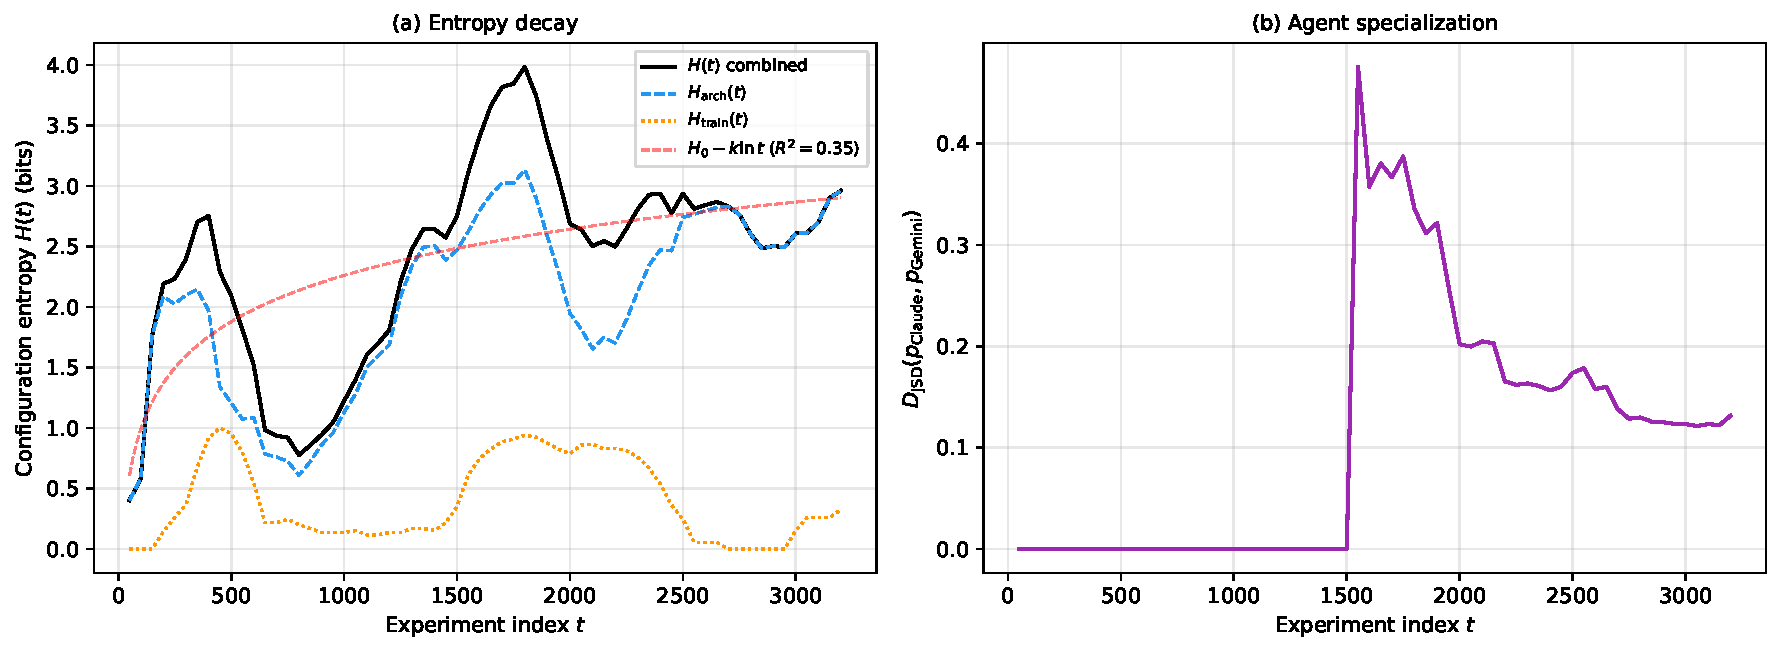
\includegraphics[width=0.95\linewidth]{figures/agent_dynamics.pdf}
\caption{Agent dynamics. (Left) Configuration-space entropy exhibits cyclic exploration-exploitation behavior. (Right) Agent specialization (JSD) decays exponentially once the second agent activates.}
\label{fig:agent_dynamics}
\end{figure}


\section{V-JEPA\,2 Discovery Trace}
\label{app:vjepa_trace}

We provide the execution trace of the V-JEPA\,2 backbone discovery to substantiate the ``autonomous web search'' claim (Section~\ref{sec:system}).

\paragraph{Step 1: Paper search via Semantic Scholar API (cycle 120, 2026-02-22 04:42).}
The Gemini agent issued live API queries including \texttt{``video foundation model 2025 2026''} and \texttt{``SigLIP2 video temporal downstream 2025''} to Semantic Scholar.
Among the returned papers, the agent identified a comparison of DINOv3 and V-JEPA\,2 feature representations for temporal tasks.
The agent's idea proposal cited this paper as \texttt{[Source: Temporal vs.\ Spatial: Comparing DINOv3 and V-JEPA2 Feature Representations]} and registered \texttt{vjepa2\_vitl} as an untried backbone (44 new backbone$\times$encoder combinations).

\paragraph{Step 2: Integration code generation.}
The agent wrote a \texttt{VJEPA2Wrapper} class (48 lines) that:
(i)~loads \texttt{facebook/vjepa2-vitl-fpc16-256-ssv2} via HuggingFace \texttt{AutoModel};
(ii)~processes 16-frame clips with stride 4 to handle variable-length dashcam video;
(iii)~mean-pools encoder hidden states to produce 1024-d clip-level features;
(iv)~concatenates clip features across the full video.
This required resolving a 768d$\to$1024d dimension mismatch with existing backbones (all other backbones output 768d or 384d), handled via the \texttt{FeatureProjection} module.

\paragraph{Step 3: Autonomous execution.}
By cycle 121, V-JEPA\,2 had 2 completed evaluations (mean AUC\,=\,0.815).
By cycle 122, 11 evaluations (mean AUC\,=\,0.851), establishing it as the top backbone.
The full pipeline---paper search, code generation, feature extraction, training, and evaluation---ran without human intervention.
All agent logs (349 research cycles, 698 log files) are included in the supplementary material.


\section{ANOVA Supporting Analysis}
\label{app:anova_support}

\paragraph{Balanced subsampling.}
To control for unbalanced group sizes, we subsample to $n = 10$ per group: balanced $\eta^2 = 0.50$ ($F = 9.83$, $p < 10^{-10}$) confirms the architecture effect.

\paragraph{Permutation test details.}
Observed $\eta^2 = 0.56$ (backbone$\times$encoder, $n = 6{,}509$) exceeds the null maximum ($\eta^2_{\mathrm{null}} \leq 0.011$, mean $= 0.005$, 99th percentile $= 0.008$), yielding $p_{\mathrm{perm}} < 10^{-4}$ (zero of 10{,}000 permutations reached the observed value). Backbone-only: $\eta^2 = 0.49$ with $p_{\mathrm{perm}} < 10^{-4}$ (null max $= 0.005$). The observed $\eta^2$ is $>$100$\times$ the null mean.

\paragraph{XGBoost surrogate.}
An XGBoost surrogate ($R^2 = 0.80$, Spearman $\rho = 0.88$ on 5-fold CV) confirms that categorical architectural features collectively account for an order of magnitude more predictive importance than continuous HPs, making no i.i.d.\ assumption.

\paragraph{Auto-sweep enrichment.}
Automated HP sweeps comprise 7.6\% of all experiments but 13.0\% of the top 100 (enrichment ratio 1.7$\times$). While HP refinement is productive, the majority of top results involve architectural choices, not automated sweeps.

\paragraph{Within-group variance and heteroscedasticity.}
Within-group variances are highly heterogeneous: VJepa2+Zipformer has within-group std $= 0.157$ ($n = 573$, CV $= 0.21$), while DINOv3-B+BiMamba has std $= 0.021$ ($n = 50$, CV $= 0.25$)---a variance ratio of $\sim$150$\times$. The standard ANOVA F-test assumes homoscedasticity; violation inflates the test statistic. We address this via: (i)~permutation ANOVA ($p_{\mathrm{perm}} < 10^{-4}$, no distributional assumptions); (ii)~XGBoost surrogate (no parametric assumptions); (iii)~the controlled cross-backbone ablation (Table~\ref{tab:xfer}), which is assumption-free. The architecture effect is confirmed by all three.

\paragraph{Non-saturating proxy robustness.}
Restricting to the 5{,}975 experiments with mAP~$< 0.999$, backbone $\eta^2 = 0.39$ [0.37, 0.41] while encoder $\eta^2 = 0.02$---architecture dominance holds. Using average precision on the non-saturated subset, backbone $\eta^2 = 0.63$ [0.61, 0.64], strengthening the signal.

\paragraph{Training loss analysis.}
Final training loss explains only 10.4\% of performance variance ($\rho = -0.14$, $R^2 = 0.10$), compared to 51\% for backbone selection. Within architecture cells ($n = 55$), mean within-cell $\rho = -0.02$.


\section{Performance Heatmap}
\label{app:heatmap}

\begin{figure}[ht]
\centering
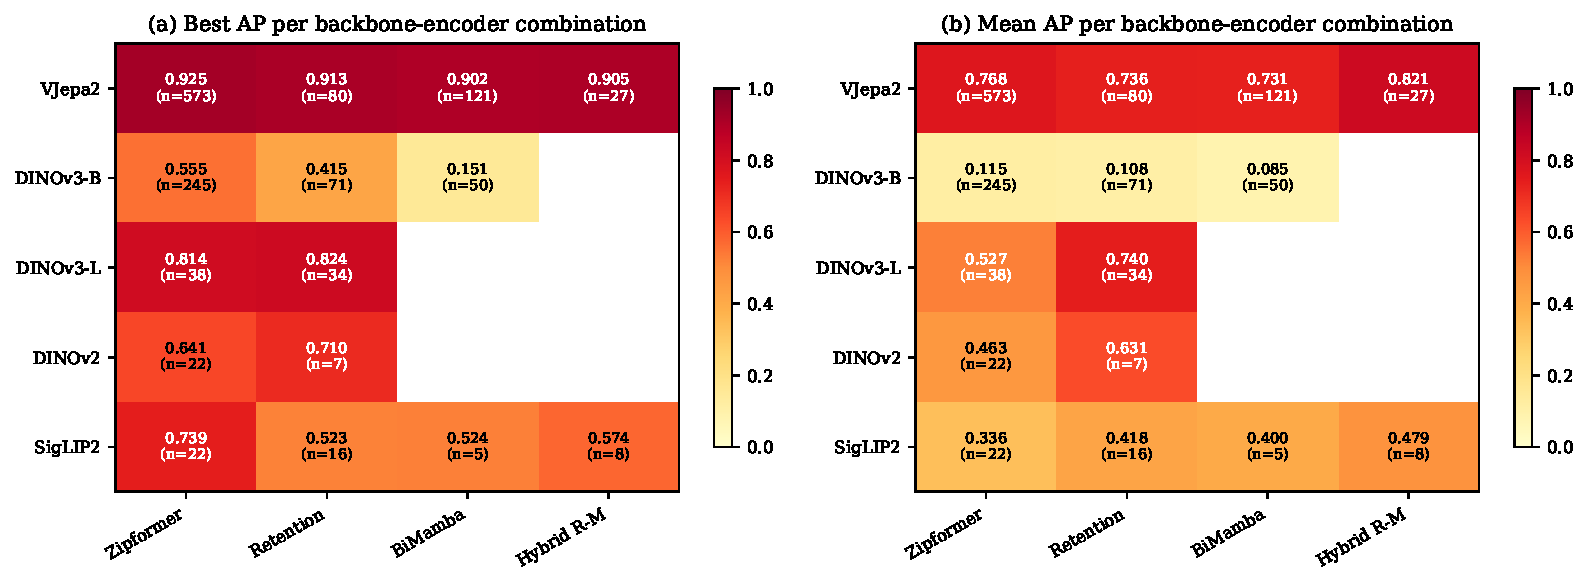
\includegraphics[width=0.9\textwidth]{figures/heatmap.pdf}
\caption{Mean AP heatmap for backbone $\times$ encoder combinations. The horizontal banding visualizes the ANOVA finding: VJepa2 dominates across all encoder types regardless of HP tuning, while DINOv3-B performs poorly across all encoders. Rows (backbones) dictate performance more than columns (encoders) or within-cell variance (HPs).}
\label{fig:heatmap}
\end{figure}


\section{Convergence Model Comparison}
\label{app:convergence_models}

We fit three functional forms to competition mAP convergence curves (Table~\ref{tab:convergence_models}). The logistic model is strongly preferred ($\Delta\text{AIC} > 100$), suggesting sigmoidal saturation. The LLM trajectory has only 11 improvement steps in 3{,}138 experiments, better characterized as a step function where each step corresponds to an architectural decision.

\begin{table}[ht]
\centering
\caption{Convergence model comparison on competition mAP. Lower AIC/BIC is better.}
\label{tab:convergence_models}
\small
\begin{tabular}{@{}llcccc@{}}
\toprule
Policy & Model & $R^2$ & AIC & BIC & $\Delta$AIC \\
\midrule
\multirow{3}{*}{TPE}
& Power-law & 0.80 & $-595$ & $-587$ & 123 \\
& Exponential & 0.92 & $-703$ & $-695$ & 15 \\
& \textbf{Logistic} & \textbf{0.93} & $\mathbf{-719}$ & $\mathbf{-710}$ & 0 \\
\midrule
\multirow{3}{*}{Random}
& Power-law & 0.86 & $-656$ & $-647$ & 161 \\
& Exponential & 0.96 & $-804$ & $-795$ & 13 \\
& \textbf{Logistic} & \textbf{0.96} & $\mathbf{-817}$ & $\mathbf{-808}$ & 0 \\
\bottomrule
\end{tabular}
\end{table}


\section{Comparison with Concurrent Work}
\label{app:concurrent}

\begin{table}[ht]
\centering
\caption{Comparison with Karpathy's concurrent autoresearch \citep{karpathy2026autoresearch}.}
\small
\begin{tabular}{@{}lcc@{}}
\toprule
Dimension & This work & Karpathy (2026) \\
\midrule
Formal framework & Yes (Defs 1, Eq 1) & No \\
ANOVA decomposition & Yes ($\eta^2 = 0.20$--$0.51$) & No \\
Experiments & 10{,}000+ & $\sim$700 \\
Tasks & 2 (collision + UCF-101) & 1 (language model) \\
Classical baselines & TPE, BOHB, Random ($n = 3{,}244$) & None \\
Obfuscated ablation & Yes ($n = 1{,}609$) & No \\
Cross-task validation & Yes & No \\
\bottomrule
\end{tabular}
\end{table}


\section{SSC vs.\ NAS Comparison}
\label{app:ssc_vs_nas}

\begin{table}[ht]
\centering
\caption{SSC vs.\ NAS: complementary approaches at different granularities.}
\label{tab:ssc_vs_nas}
\small
\begin{tabular}{@{}lccc@{}}
\toprule
Dimension & This work (SSC) & DARTS/ENAS & EvoPrompting \\
\midrule
Search level & Pretrained models + encoders & Cell topologies & Code-level NN \\
Prerequisites & Frozen or LoRA backbones & Shared weights & Fixed op vocab \\
What varies & Backbone paradigm, fusion & Cell connections, ops & Layer code \\
Cross-paradigm & Yes (SSL, CLIP, video) & No & No \\
Scale & 3{,}190+ experiments & 100--500 archs & 100--200 programs \\
\bottomrule
\end{tabular}
\end{table}


\section{Temporal Encoder Architectures}
\label{app:architectures}

The encoder dimension of $\Cspace_{\mathrm{arch}}$ comprises four families:
\textbf{Zipformer} \citep{yao2023zipformer} (multi-scale attention with BiasNorm and dynamic bypass),
\textbf{RetNet} \citep{sun2023retnet} (multi-scale retention with exponential decay),
\textbf{BiMamba} \citep{gu2023mamba} (bidirectional selective SSM), and
\textbf{Hybrid Retention-Mamba} (alternating retention and SSM layers).

\paragraph{Zipformer block.}
Three sub-layers with bypass connections:
\begin{align}
h_1 &= \mathrm{Bypass}_{\mathrm{attn}}\big(x,\; x + \mathrm{MHSA}(\mathrm{BiasNorm}(x))\big) \nonumber \\
h_2 &= \mathrm{Bypass}_{\mathrm{conv}}\big(h_1,\; h_1 + \mathrm{Conv1D}(\mathrm{BiasNorm}(h_1))\big) \\
h_3 &= \mathrm{Bypass}_{\mathrm{ff}}\big(h_2,\; h_2 + \mathrm{FFN}(\mathrm{BiasNorm}(h_2))\big) \nonumber
\end{align}

\paragraph{RetNet.}
$\mathrm{Retention}(Q, K, V; \gamma) = (QK^\top / \sqrt{d} \odot D(\gamma)) V$, where $D_{ij}(\gamma) = \gamma^{i-j}$ for $i \geq j$. Multi-scale: $H$ heads with $\gamma_h = 1 - 2^{-(5+h)}$.

\paragraph{BiMamba.}
Selective SSM: $\bar{A}_t = \exp(\delta_t A)$, $h_t = \bar{A}_t h_{t-1} + \bar{B}_t x_t$, $y_t = C(x_t)^{\!\top} h_t + D x_t$. Bidirectional extension averages forward and reversed-sequence outputs.


\section{Obfuscation Protocol}
\label{app:obfuscation}

The obfuscation map randomizes assignments to remove positional cues:

\begin{center}
\small
\begin{tabular}{@{}ll@{}}
\toprule
Obfuscated & Real \\
\midrule
Backbone\_A & DINOv3-B \\
Backbone\_B & V-JEPA\,2 \\
Backbone\_C & SigLIP2 \\
Backbone\_D & DINOv2-B \\
Backbone\_E & DINOv2-S \\
\midrule
Encoder\_1 & RetNet \\
Encoder\_2 & Zipformer \\
Encoder\_3 & BiMamba \\
Encoder\_4 & Hybrid R-M \\
\bottomrule
\end{tabular}
\end{center}

The LLM agent sees only obfuscated names in the leaderboard, rules, and schema. A transparent de-obfuscation layer maps names back to real components before training, so model quality is identical. The agent receives dimension information (768d, 1024d) but no semantic descriptions.


\section{Cost and Compute Details}
\label{app:cost}

\begin{table}[ht]
\centering
\caption{Cost and efficiency comparison. Marginal SSC cost decomposes the LLM campaign into three expansion events.}
\label{tab:cost}
\small
\begin{tabular}{@{}lcccccc@{}}
\toprule
Policy & GPU-hrs & API cost & Best mAP & mAP/GPU-hr & min/exp \\
\midrule
$\pi_{\mathrm{LLM}}$ (total) & 992 & \$2{,}000 & 0.727 & $7.3 \times 10^{-4}$ & 18.9 \\
$\pi_{\mathrm{TPE}}$ & 82 & \$0 & 0.696 & $8.5 \times 10^{-3}$ & 3.3 \\
$\pi_{\mathrm{BOHB}}$ & 58 & \$0 & 0.702 & $1.2 \times 10^{-2}$ & 6.8 \\
$\pi_{\mathrm{rand}}$ & $\sim$117 & \$0 & 0.702 & $6.0 \times 10^{-3}$ & --- \\
\midrule
\multicolumn{6}{@{}l}{\emph{Marginal SSC cost (LLM campaign decomposition):}} \\
\quad VJepa2 backbone & 219 & --- & $+0.018$ & --- & --- \\
\quad Multi-backbone fusion & 370 & --- & $+0.003$ & --- & --- \\
\quad GRU/LSTM encoders & 113 & --- & $+0.000$ & --- & --- \\
\bottomrule
\end{tabular}
\end{table}

VJepa2 backbone discovery---the single highest-impact SSC event---cost 219 GPU-hrs for a 0.018 mAP gain. Per-experiment cost difference reflects training regime: baselines use pre-extracted frozen features ($\sim$3 min/exp), while the LLM campaign includes on-the-fly feature extraction, failed experiments with auto-diagnosis, and multi-backbone fusion ($\sim$19 min/exp).


\section{UCF-101 Extended Results}
\label{app:ucf101}

\paragraph{Setup.}
Five backbones (DINOv2-S 384d, DINOv2-B 768d, DINOv3-B 768d, SigLIP2 768d, VJepa2 1024d), seven encoders (Zipformer, BiMamba, RetNet, Hybrid R-M, GRU, LSTM, Transformer). TPE ($n = 498$) and Random ($n = 499$) baselines from scratch. Two LLM agents: Claude (489 experiments, best 0.946 by experiment 10) and Gemini (501 experiments, best 0.949 by experiment 25). Both independently concentrated on SigLIP2.

\paragraph{Expanded baselines.}
Adding GRU, LSTM, and Transformer encoders ($n = 997$ total) did not change the landscape. New encoders achieved mean AP $= 0.89$ with TPE, comparable to original encoders.

\paragraph{Obfuscated ablation ($n = 596$).}
Three of five backbones share 768d. The agent included Model\_4 (SigLIP2) in 97\% of configurations (575 of 593), $4.8\times$ the uniform expectation. Dimension cannot explain this concentration---the definitive test of the performance-signal-suffices claim.


\section{Reproducibility Details}
\label{app:reproducibility}

\paragraph{Hardware and software.}
$2 \times 8$ NVIDIA H100 80GB GPUs; $\sim$1{,}000 GPU-hours (LLM) + $\sim$200 (baselines). Python 3.10, PyTorch 2.x. Features extracted by agent-written code and cached (not pre-cached by humans): V-JEPA\,2 (1024d), DINOv2 (768d), DINOv3 (768d), SigLIP2 (768d). When an agent proposes a backbone not yet cached, the system autonomously downloads weights, extracts features using the agent's integration code, and caches them.

\paragraph{LLM agents.}
Claude Opus 4 (819 cycles) and Gemini 2.5 Pro (864 cycles), both at default temperature, 3--5 base ideas per cycle. Total API cost: $\sim$\$2{,}000. System prompt template released with Orze codebase.

\paragraph{Replication artifacts.}
Code is available at the anonymized repository (see footnote 1). YAML configs for top-5 models and all baseline policies included under \texttt{configs/}. Pre-extracted feature caches for both datasets hosted on Hugging Face Datasets. Docker container provided.

\paragraph{Training protocol.}
Each experiment trains a temporal encoder on frozen backbone features for 5--30 epochs ($\sim$3--10 min/H100) with AdamW. Nexar: 1{,}500 videos (50\% positive), split 80/10/10, features at 5 fps ($T=20$).


\section{Notation Table}
\label{app:notation}

\begin{table}[ht]
\centering
\caption{Complete notation reference.}
\small
\begin{tabular}{@{}lll@{}}
\toprule
Symbol & Definition & Domain \\
\midrule
$\Cspace$ & Configuration space & $\Cspace_{\mathrm{arch}} \times \Cspace_{\mathrm{loss}} \times \Cspace_{\mathrm{train}} \times \Cspace_{\mathrm{data}}$ \\
$c$ & A specific configuration & $c \in \Cspace$ \\
$f(c)$ & Evaluation function & $f: \Cspace \to [0, 1]$ \\
$y_t$ & Observed metric at step $t$ & $y_t = f(c_t) + \epsilon_t$ \\
$\pi$ & Search policy & $\pi: (\Cspace \times \R)^* \to \Delta(\Cspace)$ \\
$H_t$ & History at step $t$ & $\{(c_1, y_1), \ldots, (c_t, y_t)\}$ \\
$\APstar(N)$ & Cumulative best & $\max_{i \leq N} y_i$ \\
$\eta^2$ & ANOVA effect size & Proportion of variance explained \\
\bottomrule
\end{tabular}
\label{tab:notation}
\end{table}


\section{Case Study: ASR Leaderboard---SSC Beyond Architecture}
\label{app:asr}

The main paper establishes that search space construction (SSC) dominates within-space optimization (WSO) when architecture variance is high.
A natural question is: \emph{what happens when architecture is fixed?}
We report a deployment of Orze on automatic speech recognition (ASR) where $\eta^2_{\mathrm{arch}} = 0$ by design---the base model is fixed, and all improvement comes through LoRA fine-tuning.
The results confirm the paper's core insight in a stronger form: even with zero architecture search, the LLM agent's value still comes from \emph{constructing} the right training configuration---not from optimizing within it.

\paragraph{Setup.}
We deployed Orze on the HuggingFace Open ASR Leaderboard (8 ESB benchmark datasets \citep{gandhi2022esb}), targeting $\leq$5.40\% average WER.
The base model is Higgs-Audio-v3-8B (Whisper-Large-v3 encoder + Qwen3-8B decoder, 8.91B parameters; baseline 6.60\% WER without fine-tuning).
The research agent (Gemini 2.5 Pro) proposes LoRA training configurations; a code agent (Claude Sonnet 4) implements strategies; the system autonomously trains, evaluates, and analyzes errors.

\paragraph{Phase 1: WSO on inference strategies ($n = 2{,}600$, 7 days).}
The agent first explored inference-time modifications: backchannel filtering, VAD-based chunking, dynamic token limits, and 180 other algorithmic strategies---all within a fixed model.
This is pure WSO: tuning decoding parameters and post-processing in a fixed configuration space.
\textbf{None improved AMI meeting WER beyond the manual LoRA baseline} (9.85\%).
Consistent with the main paper's finding, WSO within a fixed space yields diminishing returns.

\paragraph{Phase 2: SSC on training data composition ($n = 43$, 5 days).}
The breakthrough came when the agent shifted from inference-time strategies to training data composition.
Per-sample error analysis---an automated module that classifies each prediction error by pattern (backchannel deletion, hallucination, substitution)---revealed that short meeting utterances ($<$3s: ``yeah,'' ``okay,'' ``mm-hmm'') accounted for the majority of AMI errors.
The agent proposed and the system autonomously executed a series of LoRA training runs exploring a \emph{data-centric search space}: varying AMI sample count (8K--20K), short-utterance oversampling multiplier (3--10$\times$), SPGISpeech inclusion (0--10K), LoRA rank (32--128), and MLP targeting (on/off).
Error analysis feeds back into the agent's context after each run, enabling iterative refinement.

This is SSC, not WSO: the agent is not tuning hyperparameters in a pre-defined space---it is \emph{selecting which training data to include and how to weight it across 43 compositional configurations}.

\paragraph{ANOVA on training experiments.}
Table~\ref{tab:asr_anova} shows one-way $\eta^2$ for each configuration factor across all 43 completed training runs.
No single factor dominates: SPGISpeech inclusion ($\eta^2 = 0.133$), AMI sample count ($\eta^2 = 0.110$), MLP targeting ($\eta^2 = 0.085$), and oversampling multiplier ($\eta^2 = 0.069$) each contribute modestly.
The pattern mirrors the main paper's E2E LoRA regime (Section~\ref{sec:e2e}): under gradient-based adaptation, the landscape flattens and no single axis dominates.
The agent's value is \emph{compositional}---combining the right data mix with the right training configuration---rather than optimizing any single factor.

\begin{table}[ht]
\centering
\caption{One-way ANOVA ($\eta^2$) on 43 autonomous LoRA training runs. Avg WER is the 500-sample estimate across 8 ESB datasets. No single factor explains more than 13\% of variance, confirming a flat landscape where compositional decisions (SSC) matter more than individual parameter tuning (WSO).}
\label{tab:asr_anova}
\small
\begin{tabular}{@{}lccl@{}}
\toprule
Factor & $\eta^2$ (Avg WER) & $\eta^2$ (AMI WER) & Levels tested \\
\midrule
SPGISpeech samples & 0.133 & 0.056 & 0, 4K, 5K, 6K, 8K, 10K \\
AMI sample count & 0.110 & 0.085 & 8K, 10K, 12K, 15K, 20K \\
MLP targeting & 0.085 & 0.097 & off, on \\
Oversample multiplier & 0.069 & 0.098 & 3$\times$, 5$\times$, 6$\times$, 8$\times$, 10$\times$ \\
LoRA rank & 0.030 & 0.015 & 32, 64, 128 \\
\bottomrule
\end{tabular}
\end{table}

\paragraph{Full-scale results.}
Table~\ref{tab:asr_results} shows the progression from baseline to the agent's best configuration, verified on all samples.
The winning configuration (10$\times$ short-utterance oversampling, MLP targeting, rank 64, 6K SPGISpeech) reduced AMI WER from 9.85\% to 6.23\% ($-$37\% relative) and achieved 5.30\% average WER---\textbf{\#1 on the Open ASR Leaderboard} at submission time.

\begin{table}[ht]
\centering
\caption{ASR progression: baseline $\to$ manual LoRA $\to$ autonomous. All WERs are full-scale (all samples, Whisper EnglishTextNormalizer). Bold = best per column.}
\label{tab:asr_results}
\small
\begin{tabular}{@{}lccccccccc@{}}
\toprule
& AMI & E22 & GS & LS-C & LS-O & SPG & TED & VP & \textbf{Avg} \\
\midrule
8B Baseline (no LoRA) & 15.42 & 10.75 & 9.46 & 1.29 & 2.42 & \textbf{2.91} & 3.46 & 7.08 & 6.60 \\
v7 LoRA (manual) & 9.85 & \textbf{9.01} & \textbf{8.54} & 1.28 & 2.41 & 3.58 & \textbf{2.74} & 6.07 & 5.44 \\
\textbf{Orze autonomous} & \textbf{6.23} & 11.33 & 9.34 & \textbf{1.24} & \textbf{2.34} & 3.14 & 3.14 & \textbf{5.63} & \textbf{5.30} \\
\bottomrule
\end{tabular}
\end{table}

\paragraph{Trade-offs and limitations.}
The autonomous configuration improved AMI ($-$3.62pp) and 4 other datasets at the cost of E22 ($+$2.32pp) and GS ($+$0.80pp)---a training data source for E22 was unavailable during the winning run, a confound the error analysis module flagged for the next iteration.
All 500-sample estimates carry selection bias from sorted-by-duration evaluation; full-scale numbers differ by $\sim$0.5\% on average.
The 43 training runs use a single random seed each; we report this as a scope limitation consistent with the main paper's methodology.

\paragraph{Implications for the SSC/WSO framework.}
Section~\ref{sec:e2e} predicts that under gradient-based adaptation, $\eta^2_{\mathrm{arch}}$ decreases and ``classical HPO suffices.''
The ASR case partially confirms and partially refines this prediction.
\emph{Confirmed}: the landscape is flat (all $\eta^2 < 0.14$), consistent with the E2E LoRA regime.
\emph{Refined}: classical HPO suffices for tuning \emph{within} a fixed data recipe, but \emph{constructing} the data recipe (which datasets, what oversampling, which layers to train) is itself an SSC problem that classical optimizers cannot address---they lack the ability to diagnose error patterns and propose new data sources.

The ASR case thus extends the diagnostic from a binary (SSC vs.\ WSO) to a spectrum:

\begin{enumerate}[leftmargin=*, itemsep=1pt]
\item $\eta^2_{\mathrm{arch}}$ high $\to$ architecture SSC dominates. \emph{Dashcam: $\eta^2 = 0.51$.}
\item $\eta^2_{\mathrm{arch}}$ medium $\to$ SSC helps, less dramatically. \emph{UCF-101: $\eta^2 = 0.15$.}
\item $\eta^2_{\mathrm{arch}} \approx 0$, flat HP landscape $\to$ the remaining SSC value shifts to \emph{training data composition}: what to train on, and how much. \emph{ASR: all $\eta^2 < 0.14$, but 2{,}600 WSO experiments failed while 43 data-composition experiments succeeded.}
\end{enumerate}

The unifying principle: LLM agents add value by constructing the right search space---whether defined by architectures, data sources, or training procedures.
Once the space is constructed, WSO is a commodity.

\paragraph{Compute.}
Phase~1: $\sim$2{,}600 eval-only experiments ($\sim$400 GPU-hours on 8$\times$ A100 80GB).
Phase~2: 43 LoRA training runs + $\sim$150 evaluation-only runs ($\sim$600 GPU-hours).
Total: $\sim$1{,}000 GPU-hours over 13 days + $\sim$\$300 LLM API costs.

\subsection*{Extension: 1.7B Model}
\label{app:asr_1_7b}

To test whether the same methodology transfers across model scales, we repeated the Orze deployment on the 2.68B-parameter Higgs-Audio-v3 1.7B (Whisper-Large-v3 encoder + Qwen3-1.7B decoder). The 1.7B campaign ran 1{,}134 research cycles over $\sim$2.5 days on 8$\times$A100-80GB GPUs using the same multi-agent setup (research, professor, engineer).

\paragraph{Convergence trajectory.}
Figure~\ref{fig:asr_convergence} shows the 10 academically meaningful experiments that defined the 1.7B optimization trajectory (infrastructure-failure runs omitted). The agents progressed through three phases: baseline establishment (5.95\% 500-sample WER), configuration and data ablations (identifying max\_new\_tokens=2048, single-module LoRA, additional epochs, and AMI-heavy mixes as non-productive), and a learning rate breakthrough where the professor agent drove a monotonic AMI improvement: lr=$10^{-5}$ (15.82\% AMI, harmful) $\to$ $2\!\times\!10^{-5}$ (7.39\%) $\to$ $3\!\times\!10^{-5}$ (7.20\%) $\to$ $5\!\times\!10^{-5}$ (6.85\%) $\to$ $\mathbf{10^{-4}}$ (6.48\%). The winning configuration achieved 4.71\% 500-sample WER and, after full-scale verification, \textbf{5.36\% average WER---\#2 on the Open ASR Leaderboard}.

\begin{figure}[ht]
\centering
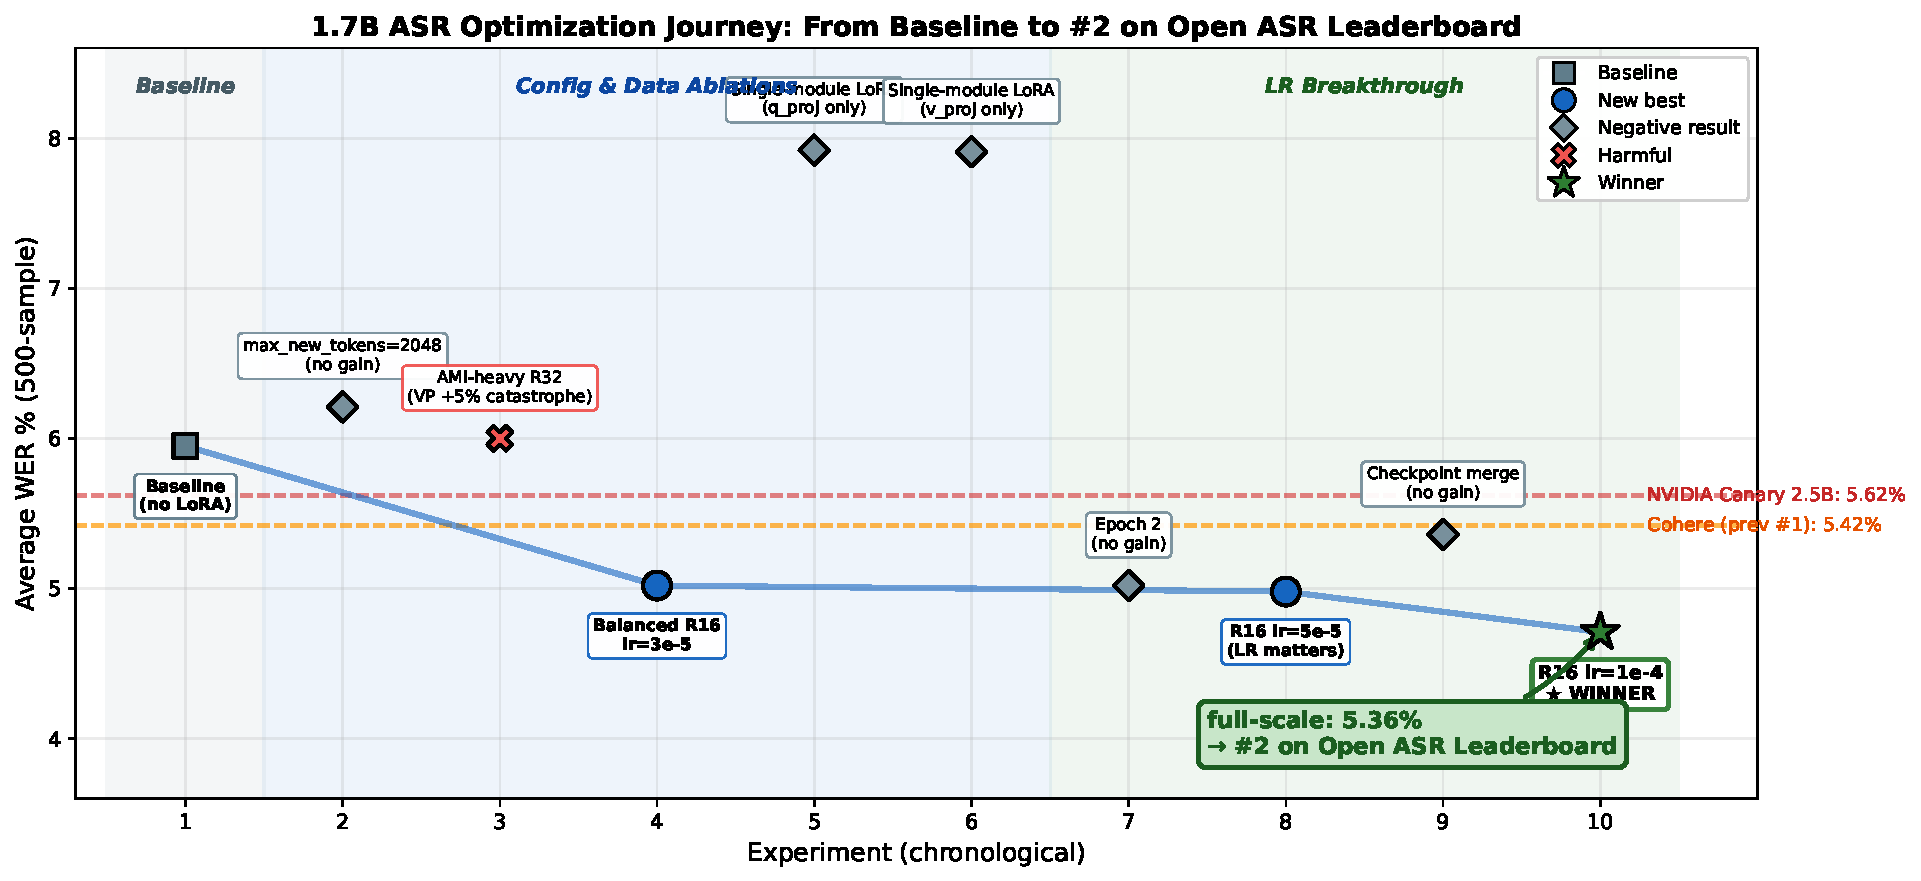
\includegraphics[width=0.9\linewidth]{figures/asr_convergence.pdf}
\caption{1.7B ASR optimization trajectory (500-sample WER). Three phases: baseline, configuration and data ablations (negative results labeled), and the learning rate breakthrough. The winning configuration reaches 4.71\% 500-sample / 5.36\% full-scale, ranking \#2. Dashed lines show prior leaderboard entries.}
\label{fig:asr_convergence}
\end{figure}

\paragraph{Evaluation calibration.}
A methodological contribution surfaced during the 1.7B campaign: across the two 1.7B full-scale evaluations we completed, 500-sample estimates underestimated full-scale WER by +0.69\% on average, with AMI contributing the largest gap (+3.21\%). The cause is that ESB datasets are sorted by duration (longest first), so the first 500 samples miss the short backchannel utterances at the tail---precisely where the model makes most AMI errors. Stratified sampling (evenly spaced indices across the full dataset) closes this gap, enabling faster iteration with more accurate full-scale projections.

\paragraph{Both models top the leaderboard.}
With the 1.7B at 5.36\% and the 8B at 5.30\%, Orze-optimized models claim \textbf{\#1 and \#2} on the HuggingFace Open ASR Leaderboard, surpassing Cohere Transcribe (5.42\%, prior \#1), Zoom Scribe (5.47\%), IBM Granite 4.0 (5.52\%), and NVIDIA Canary 2.5B (5.62\%). The 1.7B checkpoint is publicly available.\footnote{\url{https://huggingface.co/bosonai/higgs-audio-v3-stt}} The 1.7B result confirms that the SSC-on-data-composition insight from the 8B campaign transfers across scales: on a fixed architecture under LoRA fine-tuning, the dominant lever is \emph{which} training data to include and \emph{how} to weight it---not within-space hyperparameter tuning.


\end{document}
